
\documentclass{article}
\usepackage[a4paper, top=1cm, right=2cm, bottom=1cm, left=2cm]{geometry}

\usepackage[utf8]{inputenc}
\usepackage[T1]{fontenc}
\usepackage{amsmath}
\usepackage{tikz}

\title{\vspace{-2em}\Huge{\textbf{Chap 6 : Graphes}}\vspace{-1.5em}}
\author{}
\date{}

\begin{document}
    \maketitle

    \section{Introduction aux graphes}
        \subsection{Vocabulaire}
            Définition:\\
            \framebox[\textwidth][l]{Un graphe est un ensemble de sommets reliés par des arrêtes.}
        
        \subsection{Graphes complets}
        \subsection{Graphes non-orientés et chaînes}
            \subsubsection{Chaînes}
            \subsubsection{Chaîne d'Euler}


    \section{Graphes orientés et lien avec les matrices}
        \subsection{Graphes orientés}
        \subsection{Matrices}
            \subsubsection{Matrice d'adjacence}
            \subsubsection{Puissances de matrices}


    \section{Pour aller plus loin}
        \subsection{Chaîne de Markov}

        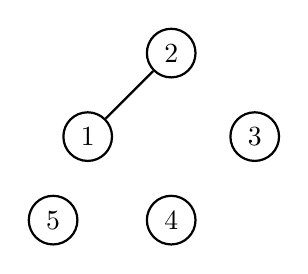
\begin{tikzpicture}[node distance={15mm}, thick, main/.style = {draw, circle}]
            \node[main] (1) {1};
            \node[main] (2) [above right of=1] {2};
            \node[main] (3) [below right of=2] {3};
            \node[main] (4) [below left of=3] {4};
            \node[main] (5) [left of=4]{5};
            \draw (1) -- (2);
        \end{tikzpicture}

        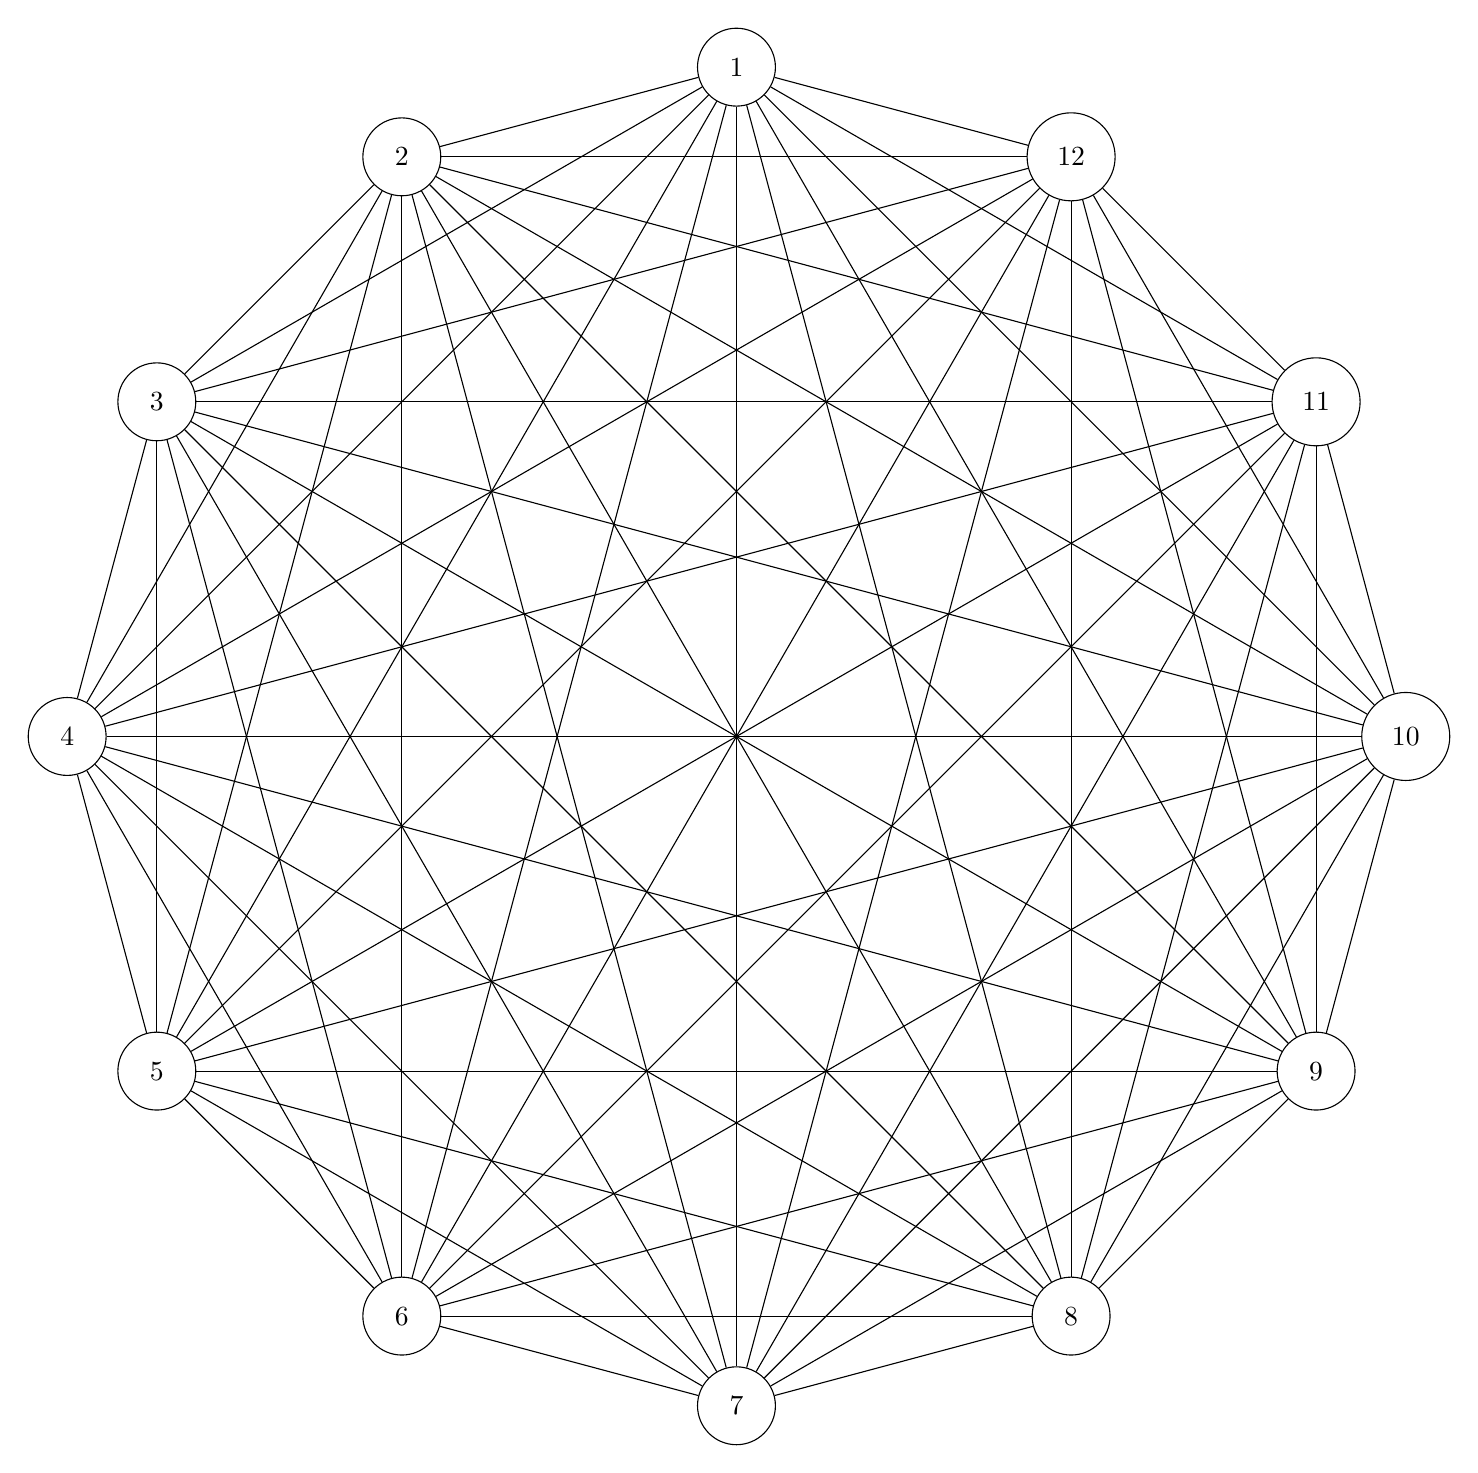
\begin{tikzpicture}[transform shape]
            \newcommand\ordre{12}
            \foreach \x in {1,...,\ordre}{
                \pgfmathparse{\x*(360/\ordre)-(360/\ordre)+90}
                \node[draw,circle,inner sep=0.25cm] (N-\x) at (\pgfmathresult:8.5cm) {\x};
            }
            \foreach \x [count=\xi from 1] in {2,...,\ordre}{
                \foreach \y in {\x,...,\ordre}{
                    \path (N-\xi) edge[-] (N-\y);
                }
            }
        \end{tikzpicture}

\end{document}
